\section{Experiments}
\label{sec:experiments}

Every table uses~\S\ref{sec:eval}: same \texttt{val\_index} order,
seed~$42$, reverse-process noise as a function of index, pairing
from~\Cref{tab:ckpts}.
VAE, concat, FiLM, and trajectory are $n{=}64$; the confirmatory
guidance dose is $n{=}256$.
The two $n$ are never pooled.

\subsection{Representation}
\label{sec:exp-rep}

Freeze each VAE and score reconstructions with no diffusion
(\Cref{tab:vae-only}).
Under \vaeone{}, $\Dec(\zlr)$ is essentially bicubic, while
$\Dec(\zhr)$ is $37.3$\,dB---well above concat \lsrmethod{}
($\approx 26.3$\,dB).
HR autoencoding is not the SR bottleneck.
\vaesr{} alignment lifts soft-decode $\mathbf{+2.33}$\,dB and LPIPS
$0.273\to 0.119$; cosine$(\zlr,\zhr)$ $0.627\to 0.790$; latent MSE
$0.584\to 0.327$.
HR recon does not move: the align term did not collapse the
autoencoder.
A suggested scale $s=1/\mathrm{std}(\mu_{\mathrm{hr}})\approx 1.065$
is not applied (\S\ref{sec:notation}).

\begin{table}[H]
  \centering
  \caption{VAE-only eval, $n{=}64$, no diffusion.}
  \label{tab:vae-only}
  \small
  \begin{tabular}{@{}lccc@{}}
    \toprule
    Method & PSNR$\uparrow$ & LPIPS$\downarrow$ & $\cos(\zlr,\zhr)$ \\
    \midrule
    Bicubic $\xup$ & $26.13$ & $0.282$ & --- \\
    \vaeone{} $\Dec(\zlr)$ & $26.15$ & $0.273$ & $0.627$ \\
    \vaesr{} $\Dec(\zlr)$ & $\mathbf{28.48}$ & $\mathbf{0.119}$ & $\mathbf{0.790}$ \\
    \vaeone{} $\Dec(\zhr)$ & $37.27$ & $0.023$ & --- \\
    \vaesr{} $\Dec(\zhr)$ & $37.28$ & $0.024$ & --- \\
    \bottomrule
  \end{tabular}
\end{table}

Retrain the same concat DDPM for $50$ epochs on each frozen VAE
(\Cref{tab:transfer}).
Soft-decode gained $+2.33$\,dB; concat SR gained $\mathbf{+0.22}$\,dB.
SR LPIPS is a tie at $\approx 0.068$.
\vaesr{} $\Dec(\zlr)$ ($28.48$\,dB) is above concat SR ($26.48$\,dB):
the sampler did not use the extra $2$\,dB (\Cref{fig:rep-gap}).

\begin{figure}[H]
  \centering
  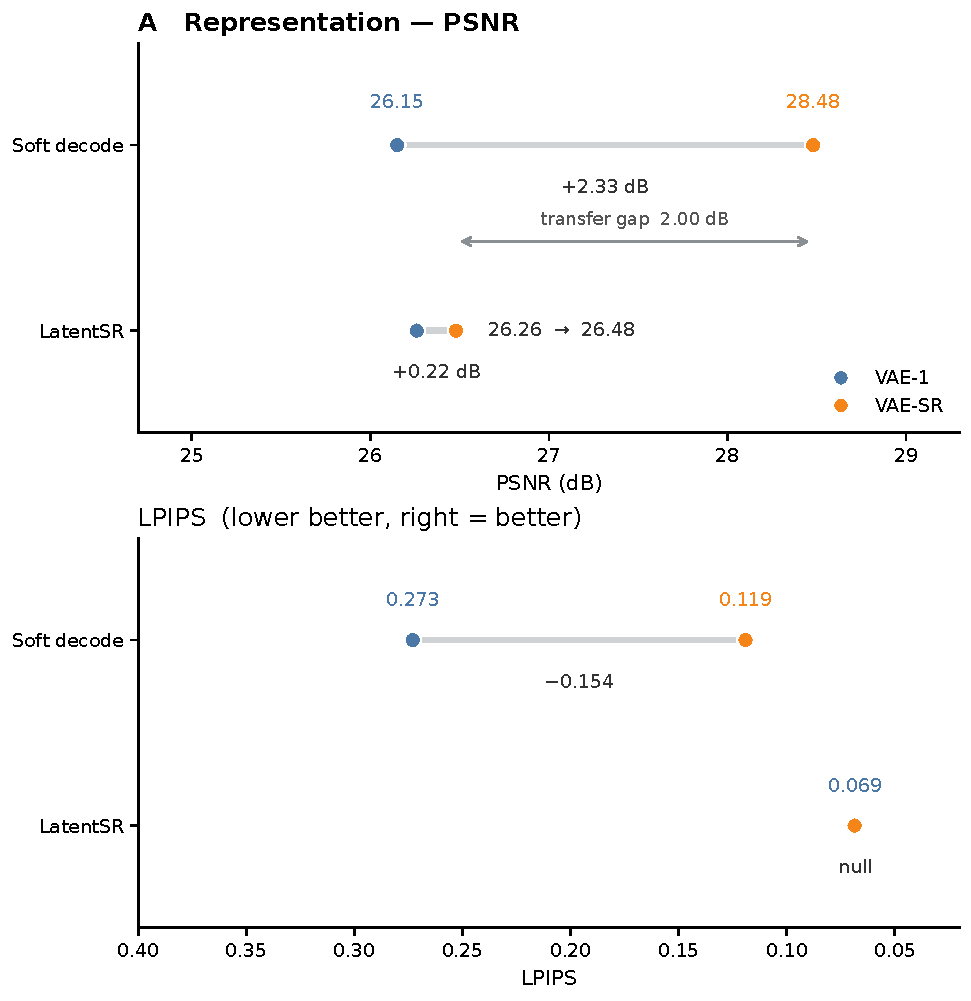
\includegraphics[width=\columnwidth]{figures/fig_a_representation.pdf}
  \caption{Representation vs.\ consumption, $n{=}64$.
  Soft-decode of $\zlr$ gains $+2.33$\,dB; concat \lsrmethod{} gains
  $+0.22$\,dB and LPIPS is a null (LPIPS axis reversed so better is
  right).}
  \label{fig:rep-gap}
\end{figure}

\begin{table}[H]
  \centering
  \caption{Matched concat / FiLM SR, $n{=}64$.
  Soft-decode is $\Dec(\zlr)$.}
  \label{tab:transfer}
  \small
  \begin{tabular}{@{}lcccc@{}}
    \toprule
     & soft PSNR & SR PSNR & soft LPIPS & SR LPIPS \\
    \midrule
    \vaeone{} concat & $26.15$ & $26.26$ & $0.273$ & $0.0683$ \\
    \vaesr{} concat & $\mathbf{28.48}$ & $26.48$ & $\mathbf{0.119}$ & $0.0685$ \\
    \vaesr{} FiLM & $28.48$ & $26.45$ & $0.119$ & $0.0696$ \\
    \bottomrule
  \end{tabular}
\end{table}

Paired tests on matched indices (\Cref{tab:paired}).
The concat $+0.22$\,dB is real and small; LPIPS is a null.
Secondary SSIM ($+0.0023$) and Sobel edge MAE ($-0.0028$) move with
PSNR.
Imagewise Spearman ($n{=}64$):
$\rho(\Delta\mathrm{PSNR}_{\mathrm{soft}},\Delta\mathrm{PSNR}_{\mathrm{SR}})=0.049$,
$\rho(\Delta\mathrm{LPIPS}_{\mathrm{soft}},\Delta\mathrm{LPIPS}_{\mathrm{SR}})=0.053$,
$\rho(\Delta\mathrm{PSNR}_{\mathrm{SR}},\mathrm{bicubic})= -0.139$,
$\rho(\Delta\mathrm{PSNR}_{\mathrm{SR}},\mathrm{HR\ Sobel})= +0.182$.
Images that gained the most in $\zlr$ did not gain more after
diffusion, so a $\lamal$ sweep is not the next question.
In latent space \vaesr{} shifts RMSE$(\zlr,\zhr)$ left while
RMSE$(\zsr,\zhr)$ overlaps \vaeone{}: the sampler lands in the same
neighborhood despite a better condition.

\subsection{Injection}
\label{sec:exp-film}

Spatial FiLM on the same frozen \vaesr{} does not close the gap
(\Cref{tab:transfer}, last row; \Cref{tab:paired}).
Train loss at epoch~$50$: concat $0.1333$ vs.\ FiLM $0.1343$
(val $0.1342$ vs.\ $0.1363$)---same plateau, FiLM slightly worse.
PSNR CI includes $0$; LPIPS is not a perceptual win.
Soft-decode is identical (same VAE).
FiLM+\vaeone{} was not trained (\S\ref{sec:method-film}).
The hole is not that the first convolution cannot see $\zlr$.

\begin{table}[H]
  \centering
  \caption{Paired tests, $n{=}64$.
  Concat row: \vaesr{} SR minus \vaeone{} SR.
  FiLM row: FiLM minus concat, both on \vaesr.}
  \label{tab:paired}
  \small
  \begin{tabular}{@{}llccc@{}}
    \toprule
    Contrast & Metric & $\Delta$ mean & $95\%$ CI & $p$ \\
    \midrule
    concat transfer & PSNR & $+0.217$ & $[+0.133,+0.300]$ & $10^{-4}$ \\
    concat transfer & LPIPS & $+0.0002$ & $[-0.0012,+0.0017]$ & $0.76$ \\
    FiLM vs.\ concat & PSNR & $-0.032$ & $[-0.089,+0.023]$ & $0.28$ \\
    FiLM vs.\ concat & LPIPS & $+0.0011$ & $[+0.0000,+0.0022]$ & $0.060$ \\
    \bottomrule
  \end{tabular}
\end{table}

\subsection{Reverse chain}
\label{sec:exp-traj}

\Cref{tab:cosine} and \Cref{fig:rev-chain} localize the miss.
\vaesr{} copies $\zlr$ mid-reverse ($\cos=\mathbf{0.985}$ at
$t{=}656$); \vaeone{} never does (peak $0.783$, coincidentally
\vaesr{}'s final number).
At $t{=}0$ most of the extra copy is gone ($0.615$ vs.\ $0.786$).
RMSE$(\zlr,\zhr)$ is constant in $t$: the VAEs differ; what changes
is the trajectory.
That is why concat and FiLM can both see a better code and still
emit nearly the same $\zsr$.

\begin{figure}[H]
  \centering
  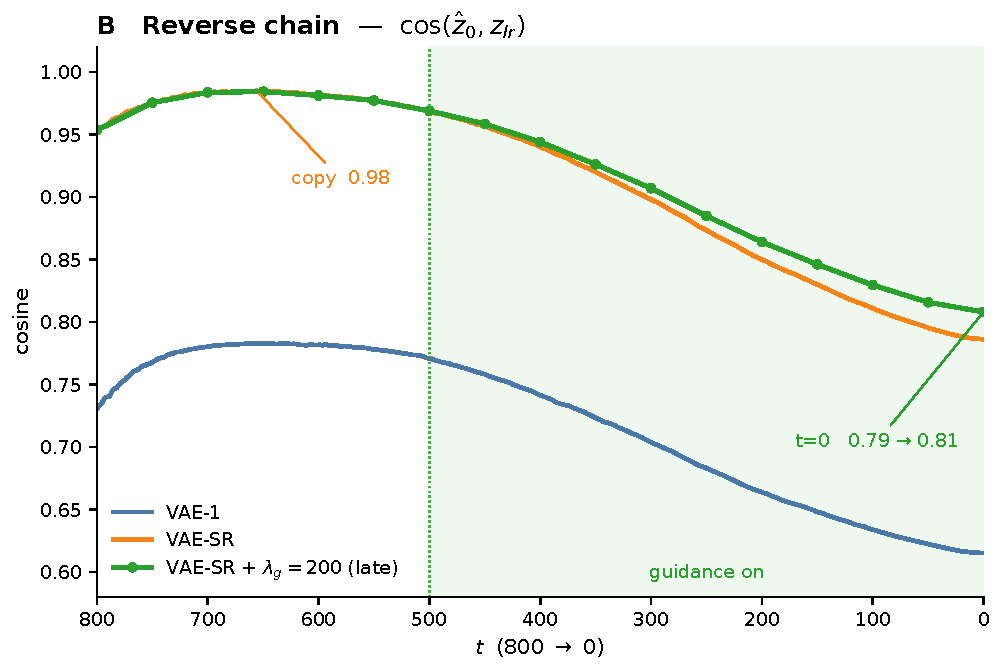
\includegraphics[width=\columnwidth]{figures/fig_b_reverse_chain.pdf}
  \caption{Reverse-chain cosine, $n{=}64$.
  \vaesr{} copies $\zlr$ near $t{=}656$ then the HR prior collapses
  the copy; late $\lamg{=}200$ ($t\le 500$) slows that collapse.}
  \label{fig:rev-chain}
\end{figure}

\begin{table}[H]
  \centering
  \caption{$\cos(\zhat(t),\zlr)$ along reverse sampling, $n{=}64$.}
  \label{tab:cosine}
  \small
  \begin{tabular}{@{}rcc@{}}
    \toprule
    $t$ & \vaeone{} & \vaesr{} \\
    \midrule
    $999$ (noise) & $0.282$ & $0.543$ \\
    $800$ & $0.730$ & $0.953$ \\
    $656$ (peak) & $0.783$ & $\mathbf{0.985}$ \\
    $500$ & $0.771$ & $0.969$ \\
    $400$ & $0.741$ & $0.940$ \\
    $0$ (clean) & $\mathbf{0.615}$ & $\mathbf{0.786}$ \\
    \bottomrule
  \end{tabular}
\end{table}

Latent cosine is not an image.
\Cref{tab:z0-img} decodes $\zhat(t)$ vs.\ $\xhr$; this is not
soft-decode $\Dec(\zlr)$.
Best absolute PSNR is near $t{=}400$ for both VAEs.
The $t{=}0$ $\Delta$ is exactly the concat $+0.22$\,dB.
Soft-decode $28.48$ is not $\Dec(\zhat)$ at the copy
($t{=}650$: $26.70$\,dB).

\begin{table}[H]
  \centering
  \caption{$\Dec(\zhat(t))$ vs.\ $\xhr$, $n{=}64$. Not soft-decode.}
  \label{tab:z0-img}
  \small
  \begin{tabular}{@{}rccc@{}}
    \toprule
    $t$ & PSNR \vaeone{} & PSNR \vaesr{} & $\Delta$ \\
    \midrule
    $800$ & $20.86$ & $22.64$ & $+1.78$ \\
    $650$ & $26.19$ & $26.70$ & $+0.51$ \\
    $400$ & $\mathbf{27.83}$ & $\mathbf{28.23}$ & $+0.39$ \\
    $0$ & $26.26$ & $26.48$ & $\mathbf{+0.22}$ \\
    \bottomrule
  \end{tabular}
\end{table}

\subsection{Guidance}
\label{sec:exp-guide}

Inference only: frozen \vaesr{} $+$ Q2 concat (\S\ref{sec:method-guide}).
Every job reprints $\mathrm{PSNR}(\Dec(\zlr),\xhr)=28.48$ on indices
$0..63$ or is discarded.

Stage~1 ($n{=}64$, $\lamg{=}200$): early $t\le 800$ and late
$t\le 500$ both reach $27.60$\,dB (\Cref{tab:stage1}).
All $64$ images gain PSNR.
LPIPS CIs include $0$ (early $p{=}0.29$, late $p{=}0.39$).
Trajectory moved: $t{=}0$ cosine $0.786\to 0.808$,
$\Lcal_g$ $0.00128\to 0.00048$---not a scale failure.
The windows tie to $0.003$\,dB; extra steps $t\in(500,800]$ lift
mid-chain $\Dec(\zhat)$ then late catches up by $t\approx 450$.
The finish comes from slowing the post-copy collapse ($t\le 500$).
Stage~2 is late-only; no combined schedule.

\begin{table}[H]
  \centering
  \caption{Stage~1 windows, $n{=}64$, $\lamg{=}200$.}
  \label{tab:stage1}
  \small
  \begin{tabular}{@{}lcc@{}}
    \toprule
    Method & PSNR & LPIPS \\
    \midrule
    Soft-decode (\vaesr) & $28.48$ & $0.119$ \\
    Unguided \lsrmethod{} & $26.48$ & $0.0685$ \\
    Early $t\le 800$ & $\mathbf{27.60}$ & $0.0695$ \\
    Late $t\le 500$ & $\mathbf{27.60}$ & $0.0693$ \\
    \bottomrule
  \end{tabular}
\end{table}

Stage~2, same $64$, late $t\le 500$, $\lamg\in\{50,200,800\}$
(\Cref{tab:dose64}, \Cref{fig:late-dose}).
Gap $28.482-26.478=\mathbf{2.004}$\,dB.
$\lamg{=}50$: smaller recon gain, LPIPS better on $\approx 80\%$ of
images.
$\lamg{=}200$: largest PSNR with no LPIPS tax---operating point.
$\lamg{=}800$: PSNR toward soft-decode, LPIPS toward $0.119$
(over-guidance).
$t{=}0$ cosine $0.786\to 0.794/0.808/0.837$: guidance does not lock
to the $0.985$ copy peak.

\Cref{tab:n256} is the pre-registered confirmation
(val\_index $0..255$, same checkpoints, late window).
Do not mix it with~\Cref{tab:dose64}.
Bars~\S\ref{sec:method-guide} all pass:
$255/256$ images gain PSNR at every $\lamg$ (sole miss:
\texttt{val\_index}~$99$, \texttt{162870.jpg});
$\Delta$LPIPS is monotone $50<200<800$;
all PSNR CIs exclude $0$.
Soft-decode on $256$ is $28.41$\,dB (first $64$ still $28.48$): extra
images, not a swapped VAE.
Gap $28.412-26.335=\mathbf{2.078}$\,dB; recovery $27\%/56\%/80\%$
matches $n{=}64$.
Unlike discovery, $\lamg{=}200$ LPIPS is significantly \emph{better}
than unguided ($p{=}0.0017$).
Operating point remains late $\lamg{=}200$: $26.33\to 27.50$\,dB
($56\%$ of the gap), LPIPS not walking to $0.119$.

\begin{figure}[H]
  \centering
  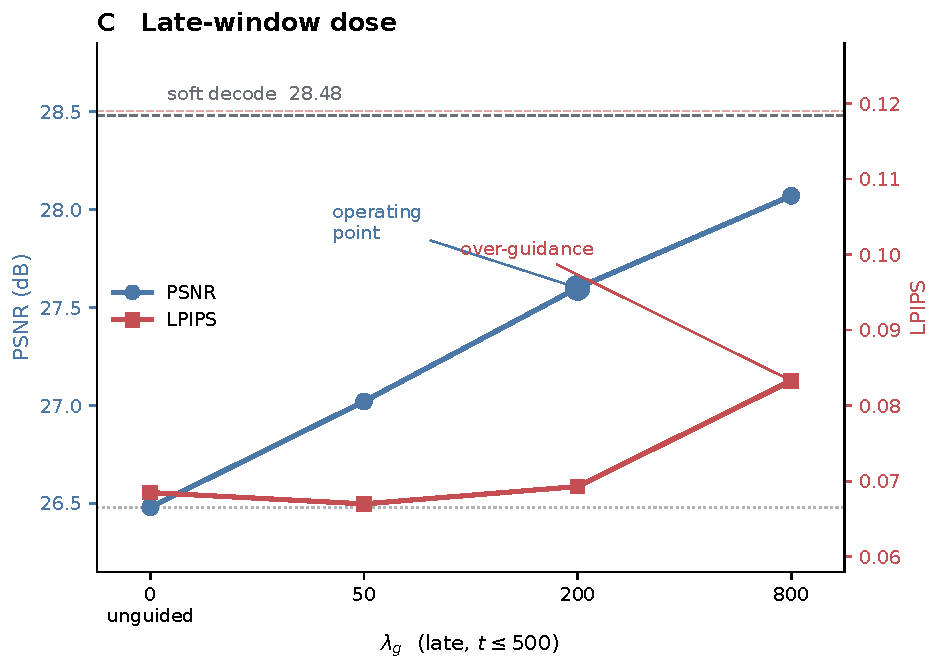
\includegraphics[width=\columnwidth,height=5.4cm,keepaspectratio]{figures/fig_c_late_dose.pdf}
  \caption{Late-window dose, $n{=}64$.
  $\lamg{=}200$ is the operating point; $\lamg{=}800$ walks LPIPS
  toward soft-decode $0.119$.
  Confirmatory $n{=}256$:~\Cref{tab:n256}.}
  \label{fig:late-dose}
\end{figure}

\begin{table}[H]
  \centering
  \caption{Late-window dose, $n{=}64$ (discovery).}
  \label{tab:dose64}
  \small
  \begin{tabular}{@{}lcccc@{}}
    \toprule
    $\lamg$ & PSNR & LPIPS & $\Delta$PSNR & $\%$ of gap \\
    \midrule
    $0$ & $26.48$ & $0.0685$ & --- & --- \\
    $50$ & $27.02$ & $\mathbf{0.0670}$ & $+0.54$ & $27\%$ \\
    $\mathbf{200}$ & $27.60$ & $0.0693$ & $+1.12$ & $\mathbf{56\%}$ \\
    $800$ & $28.07$ & $0.0833$ & $+1.59$ & $80\%$ \\
    soft-decode & $28.48$ & $0.119$ & $+2.00$ & $100\%$ \\
    \bottomrule
  \end{tabular}
\end{table}

\begin{table}[H]
  \centering
  \caption{Confirmatory late-window dose, $n{=}256$.
  $\Delta$ vs.\ unguided with $95\%$ CI.}
  \label{tab:n256}
  \small
  \begin{tabular}{@{}lcccc@{}}
    \toprule
    Method & PSNR & LPIPS & $\Delta$PSNR & $\%$ gap \\
    \midrule
    Soft-decode & $28.41$ & $0.119$ & --- & --- \\
    Unguided & $26.33$ & $0.0720$ & --- & --- \\
    Late $\lamg{=}50$ & $26.90$ & $\mathbf{0.0698}$ &
      \shortstack[l]{$+0.57$\\{\scriptsize $[0.53,0.60]$}} & $27\%$ \\
    Late $\lamg{=}200$ & $\mathbf{27.50}$ & $0.0707$ &
      \shortstack[l]{$+1.16$\\{\scriptsize $[1.11,1.22]$}} & $\mathbf{56\%}$ \\
    Late $\lamg{=}800$ & $28.00$ & $0.0832$ &
      \shortstack[l]{$+1.66$\\{\scriptsize $[1.60,1.72]$}} & $80\%$ \\
    \bottomrule
  \end{tabular}
\end{table}
